\documentclass[APA,Times1COL]{WileyNJDv5} %STIX1COL,STIX2COL,STIXSMALL

\usepackage{threeparttable}
\usepackage{dcolumn}
\usepackage{placeins}
\usepackage{subcaption}
\usepackage{graphicx}%

\graphicspath{{../Figs/}}

\articletype{Original Article}%

\received{Date Month Year}
\revised{Date Month Year}
\accepted{Date Month Year}
\journal{Real Estate Econ.}
\volume{00}
\copyyear{2025}
\startpage{1}

\raggedbottom



\begin{document}

\title{Crowded and Expensive: Density Shift as a Measure of Demand in Large US Apartment Markets}

\author[1]{Matt Larriva, CFA}

\authormark{LARRIVA}
\titlemark{Density Shift as a Measure of Demand}

\address[1]{\orgdiv{Department of Real Estate Investments}, \orgname{Brookfield Asset Management}, \orgaddress{\state{New York}, \country{United States}}}


\corres{\email{matt.larriva@brookfield.com}}

\presentaddress{250 Vesey Street, New York NY 10281 }

%\fundingInfo{Text}
%\JELinfo{ejlje}

\abstract[Abstract]{We develop a density-based demand index for rental housing and show how it segments and forecasts market behavior. Drawing on annual population‑per‑unit changes, we derive supply and demand curves for the 100 largest U.S. metropolitan areas (2010-2023) and compute each market’s implied clearing rent and inventory. By comparing these benchmarks with the actual rents and units, we classify each market-year as over- or undersupplied and over- or under-priced. These four regimes strongly predict twelve-month rent growth: undersupplied/over-priced markets see the fastest real-rent gains, while oversupplied/under-priced markets lag. Our methodology offers a clear, actionable measure of consumer housing demand, illuminates household space-vs-price trade-offs, and quantifies the ripple effects of new supply.}

\keywords{density, supply and demand, multifamily rent-growth, apartment markets}

\jnlcitation{\cname{%
\author{Larriva M.}}.
\ctitle{Density Shift as a Measure of Demand} \cjournal{\it Real Estate Econ.}
\cvol{2021;00(00):1--18}.}


\maketitle

\renewcommand\thefootnote{}
\footnotetext{\textbf{Abbreviations:} MSA, Metropolitan Statistical Area; RDI, relative density index; }

\renewcommand\thefootnote{\fnsymbol{footnote}}
\setcounter{footnote}{1}

\section{Introduction}\label{sec1}
Housing shortages and affordability concerns have risen to the forefront of policy debates in major urban markets. In the United States, housing production has consistently lagged population growth for decades, contributing to an estimated national shortfall of 4.4 million housing units \cite{betancourt2022us}. Nearly half of U.S. renter households now spend over 30\% of their income on housing \cite{censusNearlyHalf}, and from 2000 to 2024, the consumer price index (CPI) for shelter exceeded the CPI for all other items by 30\% \cite{stlouisfedConsumerPrice}. At the same time, select high-growth regions have recently experienced rent declines due to a glut of new supply \cite{mott2024ThisRegion}. This juxtaposition of chronic national undersupply with localized oversupply underscores a deeper issue: the lack of a reliable metric to measure consumer housing demand.

Traditional indicators of demand in multifamily real estate, such as occupancy rates and net absorption, are informative but fundamentally supply-constrained. Occupancy rates are naturally bounded at 100\%, and absorption cannot exceed the rate of new deliveries \cite{mueller1999real}. These constraints obscure excess demand: when all available and affordable units are occupied, latent demand becomes invisible to market participants and researchers alike \cite{gabriel2001rental, sirmans1991determinants, pyhrr1999real}. This problem inhibits clear attribution of rent increases to supply versus demand dynamics \cite{pennington2021does, molloy2022housing}. Moreover, ongoing academic debate persists around whether rising rents in constrained markets result more from supply-side limitations \cite{saiz2010geographic} or from heightened demand for desirable locations \cite{davidoff2015supply}. Without a transparent, consistent demand-side metric, attempts to assess equilibrium conditions remain incomplete.

In this paper, we introduce a novel empirical measure of rental housing demand: the \textit{rental density index} (RDI), defined as the number of people per existing rental unit in a given metropolitan area. Unlike occupancy or absorption, RDI is not inherently bounded and therefore can reflect intensifying demand even in fully occupied markets. The conceptual foundation is straightforward: as rents rise, renters economize on space---whether by delaying household formation, taking on roommates, or crowding---thus increasing the ratio of people per rental unit. By observing shifts in RDI over time, we capture underlying demand pressures that traditional metrics obscure.

Present trends support this reframing of demand, as density, rental prices, and rental preferences have all shifted meaningfully. For most of its history, the U.S. was less densely populated than its high-income peers, but in 1992 this changed. In that year, the US grew to 28 people per square kilometer, outpacing the High Income countries whose average was 23 people per square kilometer \cite{worldbankPopDensity}. The most recent figures report the US with a density of 36 and the High Income nations with an average density of 27.  Over this same period, rental prices have outpaced both wages and non-shelter inflation \cite{feiveson2024rent, stlouisfedConsumerPrice}, with younger cohorts increasingly preferring rental housing \cite{fanniemaeConsumersFeeling}.

Prior literature in urban economics and real estate has studied density extensively, often linking increased geographic density to higher wages, rents, and productivity due to agglomeration effects \cite{titman2024city, liu2018vertical}. However, these studies generally define density in terms of spatial density: people per square mile or  apartments per square mile. Our focus differs: we define density as the quotient of population over occupied rental units, which provides a clearer window into the number of people actively competing for housing. Unlike geographic density, this measure is directly responsive to shifts in demand, especially during periods of supply constraint or shocks. 

Our framework builds on the standard assumption that, all else equal, households derive higher utility from larger living spaces \cite{muth1969cities,molloy2022housing}. In high-rent markets, however, the extra price per square foot may eventually exceed the marginal benefit of additional space. To economize, renters may respond by sharing units (adding roommates), downsizing to smaller apartments, or relocating to less expensive regions. Conversely, when real rents fall or new supply comes online, the marginal cost of extra space might drop below its marginal utility, enticing households to spread out, move to larger units, or reduce unit‐share.The aggregate effect of these choices combined with the new supply additions or subtractions determines the direction the Rental Density Index change. Because the RDI directly captures these space‐consumption margins, year‐over‐year changes in RDI proxy for shifts in aggregate housing demand at prevailing prices.

\begin{figure}[htb!]
	\centerline{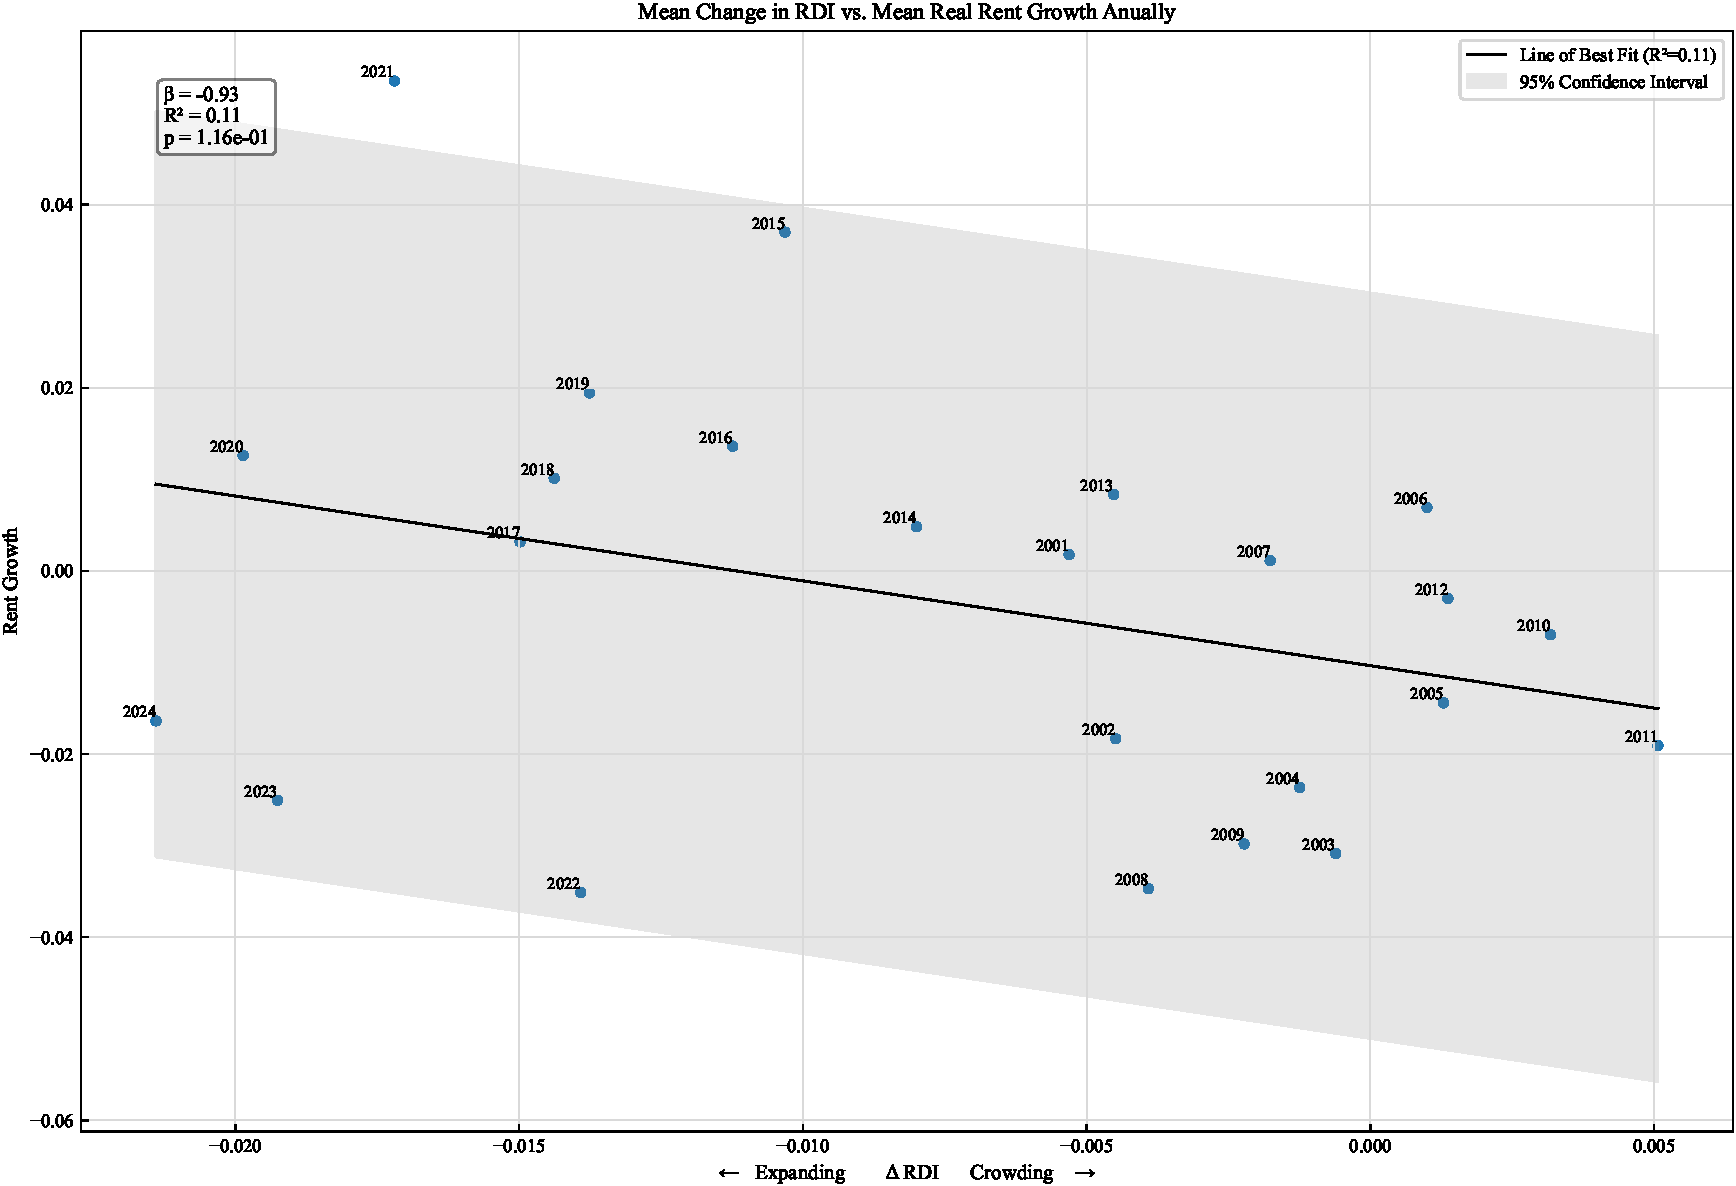
\includegraphics[height=20pc]{rdi_rent_growth_2024.pdf}}
	\caption{Relationship between annual change in Rental‑Density‑Index (horizontal) and annual real rent growth (vertical) across the 100 largest MSAs in 2024. Slope = 0.41 (p < 0.01).\label{fig:rdi_national}}
\end{figure}

Focusing on a panel of the 100 largest metropolitan statistical areas (MSA), their population, rental unit count, and change in rent, we estimate implied demand of each MSA at each of 10 years from 2013 to 2023. We plot this against rent to derive a demand curve. We then take the observed supply growth of each MSA and plot it against rent to derive a supply curve. The intersection of those two curves is the derived point of supply and rent equilibrium. Comparing a market's actual rent to the market's derived rent suggests over or underpricing. Comparing a market's actual supply growth to the market's derived supply growth provides evidence of over or undersupply. We show that by segmenting markets as over or undersupplied and over or underpriced each year, we can effectively forecast the market's next-year rent growth.  

This empirical strategy reveals consistent rent growth differences across market classifications. We find that markets classified as both overpriced and undersupplied experience significantly higher next-year rent growth than those that are underpriced and oversupplied. Specifically, markets in the former category averaged next-year relative real rent growth approximately 1.25\% higher than those in the latter category. These findings suggest that density-based classifications have predictive power and reflect latent demand more accurately than traditional indicators alone.

Our paper makes two principal contributions. First, we introduce the Rental Density Index (RDI), a novel, supply‑unbounded metric of housing demand that can be computed at scale from readily available population and unit‐stock data. Second, we demonstrate RDI’s empirical value: it not only uncovers market disequilibrium but also delivers out‑of‑sample forecasts of twelve‑month rent growth with statistically significant accuracy.

These findings carry immediate applications for all housing‐market stakeholders. For policymakers, RDI functions as an early‑warning gauge of emerging shortages, enabling targeted zoning reforms, calibrated subsidy programs, or expedited permitting in precisely those submarkets under the greatest pressure—and subsequently measuring the efficacy of those measures. Institutional investors and residential developers can embed RDI trends into feasibility and risk models, avoiding the twin hazards of overbuilding in cooling metros or underbuilding in tightening ones. Finally, RDI sharpens the housing‐affordability debate by identifying the locales where rent increases are most likely to outstrip income growth, thereby guiding tenant‐protection policies, rent‐assistance programs, and other affordability interventions to the communities that need them most.

In the next section we discuss research on other measures of demand before presenting details on our proposed variable. The Data and Descriptive Statistics section describes and analyzes the density data we used, while the Empirical Analysis section presents evidence and illustrates statistical tests performed to evaluate the validity of the classifications. The final sections discuss the results of our tests before concluding with implications and further research suggestions. 

\section{Background and Literature Review}\label{sec2}

The multifamily housing market has long relied on a narrow set of demand indicators, notably occupancy rates and net absorption. These indicators, while intuitively appealing and widely used by practitioners, are fundamentally constrained by the available stock of housing units. Occupancy rates cannot exceed 100\%, and net absorption can never exceed new supply \cite{mueller1999real, gabriel2001rental}. Consequently, they fail to capture periods of latent demand where tenants cohabitate. \cite{sirmans1991determinants, pyhrr1999real}. Occupancy in particular has become an especially measure of demand since the advent of algorithmic pricing systems. So-called revenue management systems adjust rent pricing with the goal of keeping occupancy very near 96\%, \cite{calder2024coordinated} the result of which is a variable with little signal. 

This measurement limitation is consequential. Numerous empirical studies find that real rent growth often occurs in periods of high occupancy, yet they typically ascribe this to supply constraints rather than to excess demand \cite{goodman1992rental, wheaton1991realestate}. While such studies validate the predictive value of these metrics, their theoretical bounds limit their explanatory reach, particularly when trying to assess equilibrium or derive true demand elasticities \cite{pennington2021does, molloy2022housing}.

Alternative approaches to measuring demand have included econometric estimates of demand elasticity \cite{green2002measuring}, consumer preference surveys \cite{malpezzi1996rent}, and utility-based choice models \cite{rosenthal1997housing}. However, these methods either lack the spatial and temporal granularity needed for policy or investment use, or they are not publicly available in standardized formats.

The broader urban economics literature has focused on density as a related but distinct construct. Seminal work by \cite{glaeser2001cities} and \cite{duranton2004micro} positions geographic density---typically measured as people or housing units per square mile---as a proxy for agglomeration benefits. These studies find that higher density correlates with increased productivity, innovation, and wages. However, they stop short of using density as a direct measure of housing demand.

More recent research has explored density in the context of housing affordability. \cite{ahlfeldt2019economic} and \cite{albouy2015driving} argue that densification can both alleviate and exacerbate affordability issues, depending on its implementation. For instance, densification may increase supply and reduce rents in the long term but may also create localized price pressures or quality-of-life tradeoffs that drive demand elsewhere.

Our work contributes to this literature by redefining density as \textit{people per rental unit}, rather than per geographic area. We call this the Rental Density Index (RDI). This formulation allows demand to exceed supply in a measurable way: if population grows faster than units, density rises. If renters prefer space and are observed to cohabitate only at higher prices, then shifts in RDI reveal the slope of the underlying demand curve \cite{muth1969cities, molloy2022housing}.

Unlike geographic density, which may be influenced by zoning and land use policy, RDI responds directly to demographic pressures and consumer decisions. Its changes over time---\( \Delta \text{RDI} \)---can be interpreted as demand shocks, analogous to shifts in labor force participation or consumption behavior in macroeconomic models. By linking \( \Delta \text{RDI} \) to rent outcomes, we recover a market-clearing framework that identifies over- and under-supplied markets and projects likely rent growth trajectories.

This approach also aligns with emerging calls in the real estate literature to develop forward-looking, demand-side indicators that complement the traditional focus on supply elasticity \cite{glaeser2019rethinking}. In contrast to existing studies, our method uses widely available data---population, rental unit inventory, and rent---to produce a scalable, repeatable measure of housing demand at the metro level.

In sum, our contribution lies in reinterpreting a well-studied spatial metric---density---through the lens of consumer housing decisions. By focusing on the population-to-unit ratio rather than geographic dispersion, we provide a new empirical tool to better understand and forecast real estate market dynamics.

\section{Data and Descriptive Statistics}\label{sec3}
Our data are sourced primarily from Costar and supplemented with inflation measures from the U.S. Bureau of Labor Statistics. We restrict our analysis to the 100 largest U.S. metropolitan statistical areas (MSAs) by multifamily inventory as of 2001, ensuring robust sample representation and consistency over time.

To normalize pricing data across time, we convert all nominal rent figures into real terms using the Consumer Price Index for All Urban Consumers (CPI-U), all-items, provided by the BLS. Although MSA-level inflation indices excluding rent would be ideal, such data are unavailable at a consistent and granular level for our study period. Therefore, real effective rent per square foot and rent growth metrics are adjusted using national CPI. 

We convert the rent growth figures to nominal as well, by subtracting the annual growth in CPI. Finally, we standardize the figures by subtracting the year's median rent growth. We do this to remove the impact of national macroeconomic shocks (i.e., COVID-19). This also serves to stationarize the data and remove the autoregressive tendencies of timeseries data.

Our novel demand variable, the Rental Density Index (RDI), is calculated by dividing population by rental inventory at the MSA level. We compute its year-over-year percentage change---\(\Delta\text{RDI}\)---to reflect demand dynamics more accurately. This measure avoids the bounded structure of traditional demand indicators like occupancy and absorption, which cap at 100\%.

Other variables include supply growth, computed as the ratio of delivered units to the previous year's inventory, and lagged variables prior-year rent growth. 

Importantly, no records were discarded during preprocessing. Our dataset retains all 100 MSAs over all years between 2000 and 2024. Some records are extreme, such as post-Katrina New Orleans, but we preserve fidelity to real-world dynamics by keeping them.

\begin{table*}[hbt]%
\centering
\caption{Key variables used in the empirical analysis.\label{tab:variables}}%
\begin{tabular*}{\textwidth}{@{\extracolsep\fill}ll@{\extracolsep\fill}}%
\toprule
\textbf{Variable} & \textbf{Description} \\
\midrule
\texttt{CPI}					& Consumer Price Index for All Urban Consumers: All Items in U.S. City Average \\
\texttt{real\_rentpsf}               & Costar's Rent Per Square Foot divided by indexed \texttt{CPI}\\
\texttt{real\_rent\_growth}          & Costar's Effective Rent Growth 12M less Annual percent change in \texttt{CPI} \\
\texttt{relative\_real\_rent\_growth}          & \texttt{real\_rent\_growth} less that year's median \texttt{real\_rent\_growth}\\
\texttt{inventory}             & Existing multifamily rental stock \\
\texttt{delivered}             & Units delivered in the current year \\
\texttt{pop}                   & Total MSA population (Costar/Moody’s) \\
\texttt{RDI}			       & Population divided by rental inventory \\
\texttt{delta\_RDI}	           & Year‐over‐year percentage change in \texttt{RDI} \\
\texttt{supply\_growth}        & Delivered units as \% of prior year's \texttt{inventory}\\
\bottomrule
\end{tabular*}
\end{table*}


\subsection{Variable Construction}
The key outcome variable in this study is the \textit{Rental Density Index} (RDI), calculated as the total population divided by the number of rental housing units in a given MSA-year:

\begin{equation*}
	\text{RDI}_{it} = \frac{\text{Population}_{it}}{\text{Rental Units}_{it}}.
\end{equation*}
	
Within the 100 MSAs in the study,this metric ranges from 6.8 to 64.8. It reflects the number of people per rental unit. 
\begin{figure*}[hbt!]
	\centering
	
	\begin{subfigure}[b]{0.32\textwidth}
		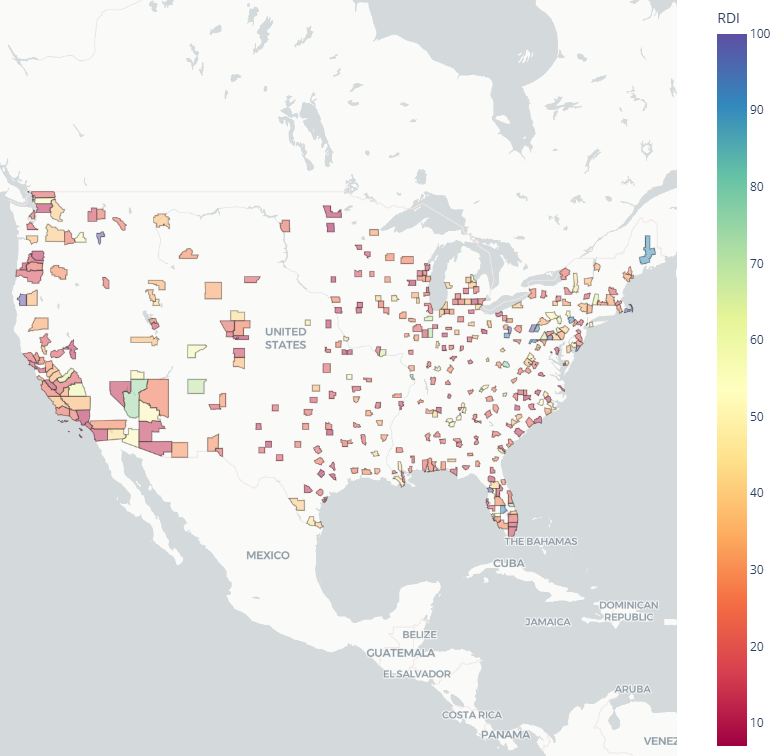
\includegraphics[width=\linewidth]{us.png}
		\caption{United States}\label{fig:us_choropleth}
	\end{subfigure}\hfill
	\begin{subfigure}[b]{0.32\textwidth}
		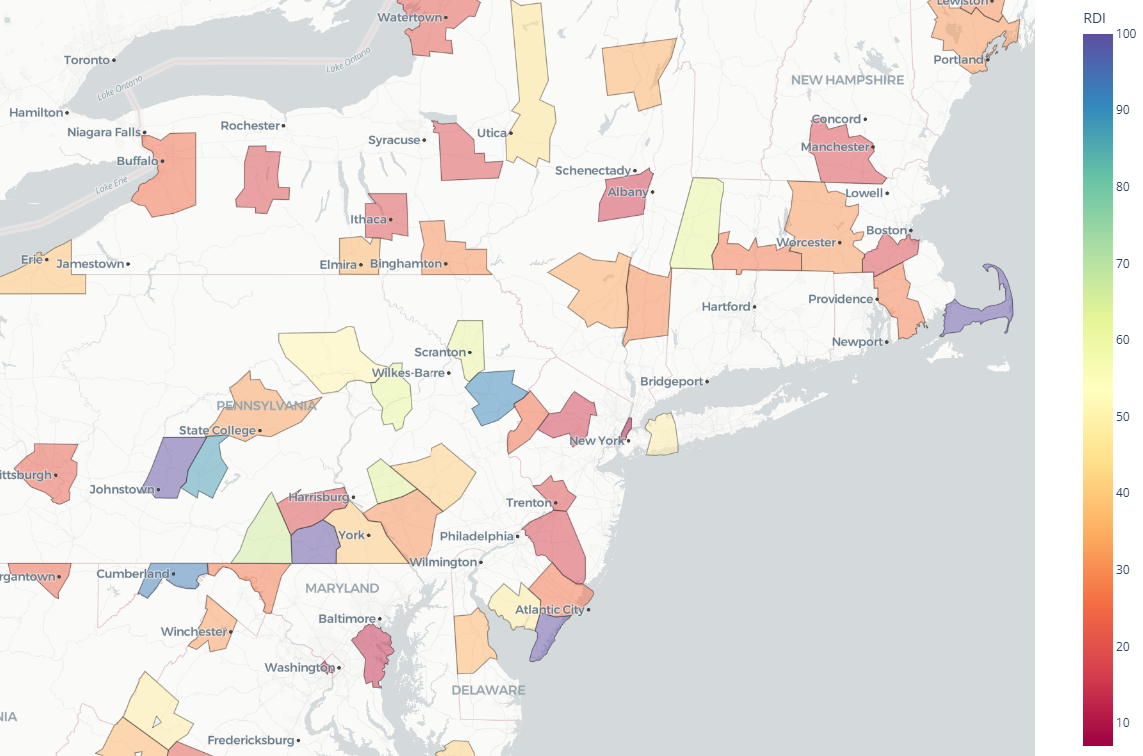
\includegraphics[width=\linewidth]{tristate.png}
		\caption{Tri‑State area}\label{fig:tristate_choropleth}
	\end{subfigure}\hfill
	\begin{subfigure}[b]{0.32\textwidth}
		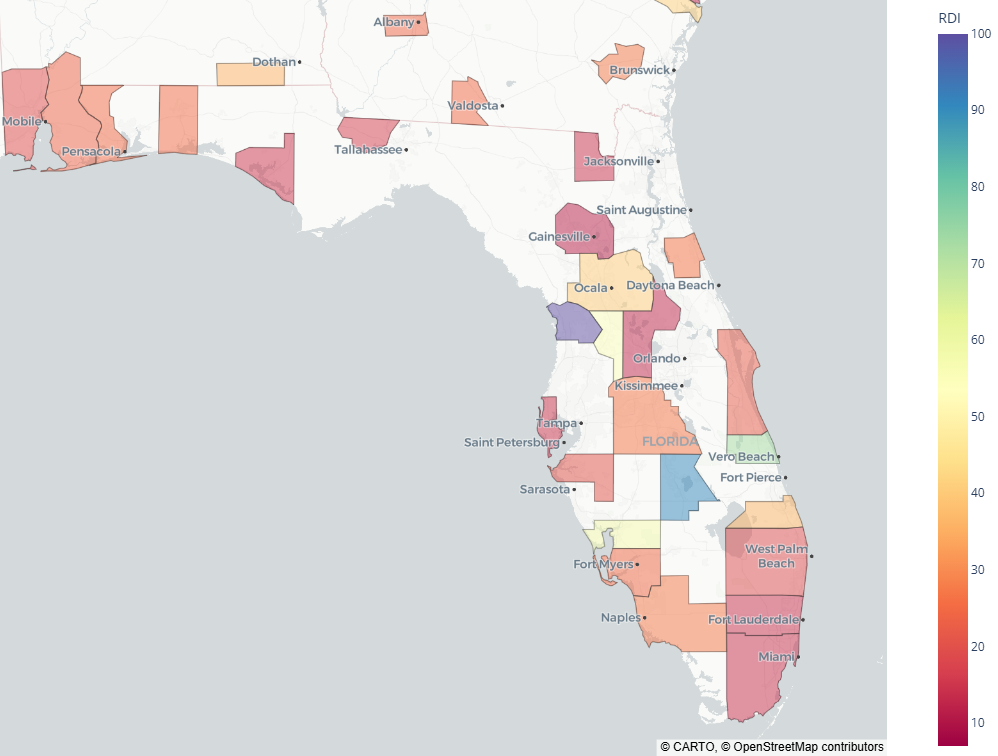
\includegraphics[width=\linewidth]{florida.png}
		\caption{Florida}\label{fig:florida_choropleth}
	\end{subfigure}
	
	\caption{Rental‑Density‑Index (RDI) choropleths at three spatial scales.}
	\label{fig:choropleth_panel}
\end{figure*}


While the RDI itself is useful for identifying how tight a market is at a given point in time, its absolute level is shaped by long-run demographic and structural trends such as rentership rates and changes in household formation. Accordingly, we focus on the \textit{year-over-year change in RDI}:

\begin{equation*}
	\Delta \text{RDI}_{it} = \text{RDI}_{it} - \text{RDI}_{it-1}.
\end{equation*}

The RDI and can move sharply in times of natural disasters, as shown by the figures in table \ref{tab:extremes}, but so can real rent growth.  

\begin{table}[ht]
	\centering
	\caption{Extreme observations in RDI and real rent growth}
	\label{tab:extremes}
	\begin{tabular}{lllrcrr}
		\toprule
		Category & Year & MSA & Population & Inventory & RDI & Real rent growth \\
		\midrule
		Highest RDI                   & 2001 & Long Island-NY           & 2,785,876 &  43,235 & 64.435 & -0.0079     \\
		Lowest RDI                    & 2024 & Fargo-ND                 &   264,314 &  38,634 &  6.841 & -0.0128      \\
		Highest real rent growth      & 2006 & New Orleans-LA           & 1,055,155 &  57,719 & 18.281 & 0.2809   \\
		Lowest  real rent growth      & 2005 & New Orleans-LA           & 1,300,912 &  57,679 & 22.554 & -0.1915  \\
		\bottomrule
	\end{tabular}
\end{table}



The change in RDI (\( \Delta \text{RDI} \)) offers several advantages. First, it mitigates issues of nonstationarity in the level RDI, enabling cross-market comparison. Second, it reduces the impact of varying rentership percentages across cities. Most importantly, \( \Delta \text{RDI} \) captures demand pressure on housing stock: when it rises, it indicates more people are consolidating into fewer rental units, signaling tightening demand. When it falls, it implies renters are spreading out and absorbing more space, suggesting slack.

Theoretically, under the assumption that renters prefer more space to less, the change in RDI reveals when prices are sufficiently high to induce cohabitation and when price relief allows individuals to live separately. Thus, \( \Delta \text{RDI} \), especially when combined with rent growth, helps identify periods of excess demand or slack and allows us to trace out implied demand curves. As we show later, this approach allows us to locate the intersection between demand and supply curves using observable outcomes.


\subsection{Summary Statistics}
Table \ref{tab:summary_stats} provides descriptive statistics for the key variables across the full panel. On average, the RDI across all MSAs and years is approximately 2.31 persons per rental unit, with a standard deviation of 0.35. The average real rent per square foot is \$1.22, and the average annual growth in rental supply is 1.9\%. The missing records exist only in the beginning or ending years as the prior period and next-period values do not exist. 

\begin{table}[hbt!]
	\centering
	\caption{Summary Statistics (2000--2024)}\label{tab:summary_stats}
	\begin{tabular}{lrrrrrrrr}
	\toprule
	Variable & Mean       & Std.\ Dev.\   & Min       & 25th Pct.  & Median     & 75th Pct.  & Max        & Missing \\
	\midrule
	Population          & 2,012,976  & 2,169,231  &   175,653  &   758,060  & 1,224,731  & 2,422,333  & 14,849,020 &   0  \\
	Inventory           &   133,435  &   190,354  &    20,783  &    35,735  &    66,261  &   153,774  &  1,572,425 &   0  \\
	Supply growth       &      0.0169&      0.0152&     –0.0173&     0.0057 &    –0.0059 &     0.0239 &     0.1061 & 100  \\
	RDI                 &     18.259 &      6.852 &      6.841 &    13.737  &    17.067  &    20.967  &    64.795  &   0  \\
	RDI growth          &     –0.0078&      0.0151&     –0.1895&    –0.0163 &    –0.0059 &     0.0022 &     0.0512 & 100  \\
	Real rent (\$/sqft) &      0.9489&      0.3551 &      0.5584&     0.7164 &     0.8373 &     1.0436 &     2.9110 &   0  \\
	Real rent growth    &     –0.0035&      0.0300 &     –0.1915&    –0.0215 &    –0.0046 &     0.0114 &     0.2809 & 100  \\
	\bottomrule
\end{tabular}
\end{table}

\subsection{Coverage and Representativeness}
The sample includes approximately 1,300 MSA-year observations, covering a mix of large coastal cities, fast-growing Sun Belt metros, and slower-growing Midwestern regions. Together, these MSAs account for over 16 million of the 22 million U.S. apartment units, providing a representative snapshot of national rental dynamics. 

\subsection{Preliminary Observations}

Figure \ref{fig:sidebyside} traces the national Rental Density Index (RDI) from 2000 to 2024. Contrary to conventional wisdom about an acute housing shortage, we observe a steady decline in people per unit (from roughly 16 people-per-unit in 2000 to 13 people-per-unit in 2024). A companion histogram of ΔRDI is stationary but skewed slightly negative, confirming that most years see more units added per new person than vice versa.

\begin{figure}[!htb]
	\centering
	\begin{subfigure}[b]{0.48\textwidth}
		\centering
		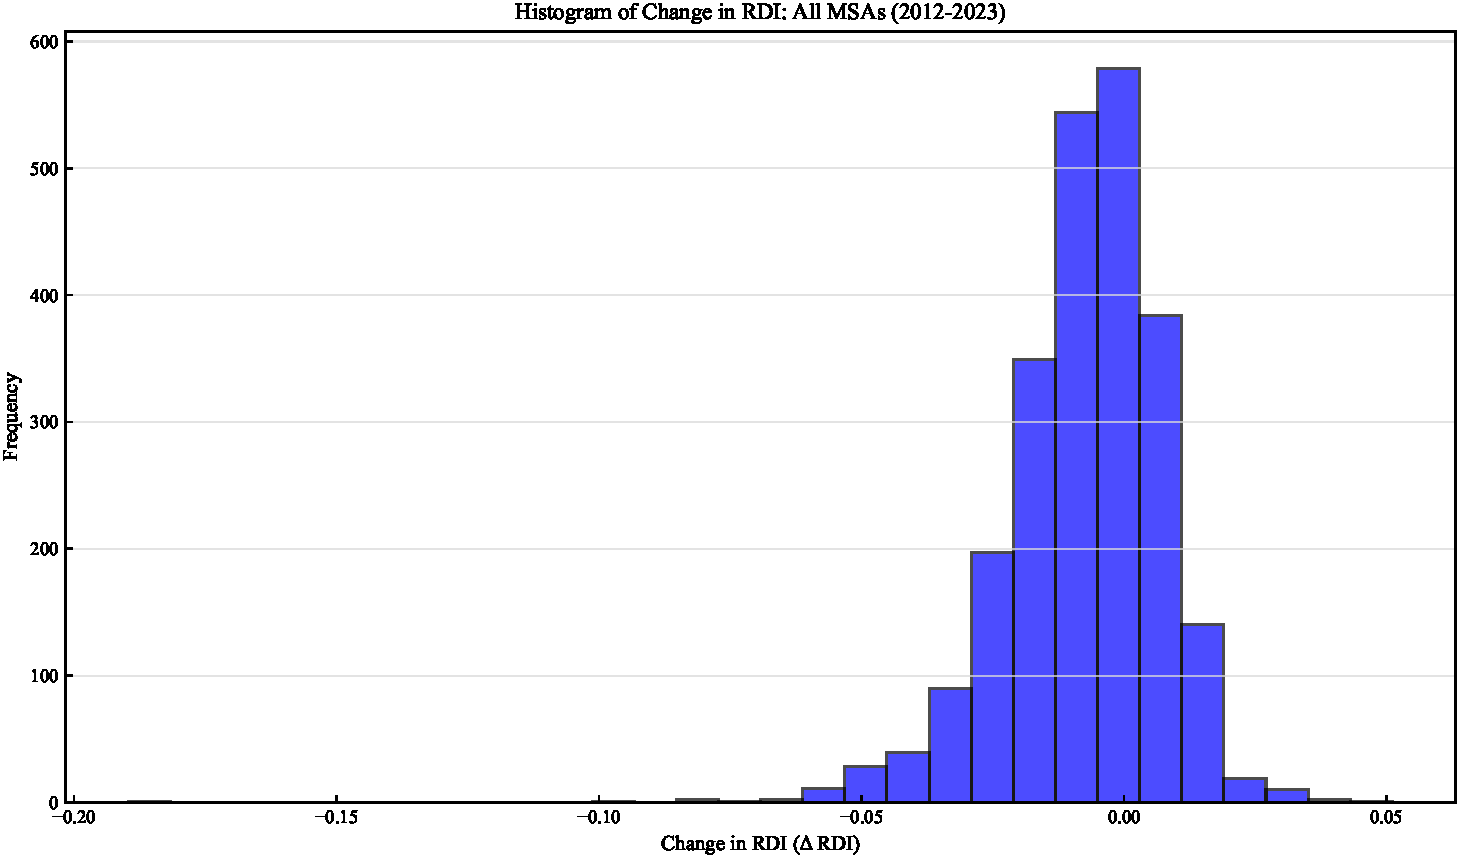
\includegraphics[width=\textwidth]{rdi_growth_histogram.pdf}
		\caption{A histogram of the annual change in RDI across 100 MSAs in the years 2001-2023. The outlier to the left is New  Orleans in 2004, due to Huricane Katrina.\label{fig:rdi_hist}}
	\end{subfigure}
	\hfill
	\begin{subfigure}[b]{0.48\textwidth}
		\centering
		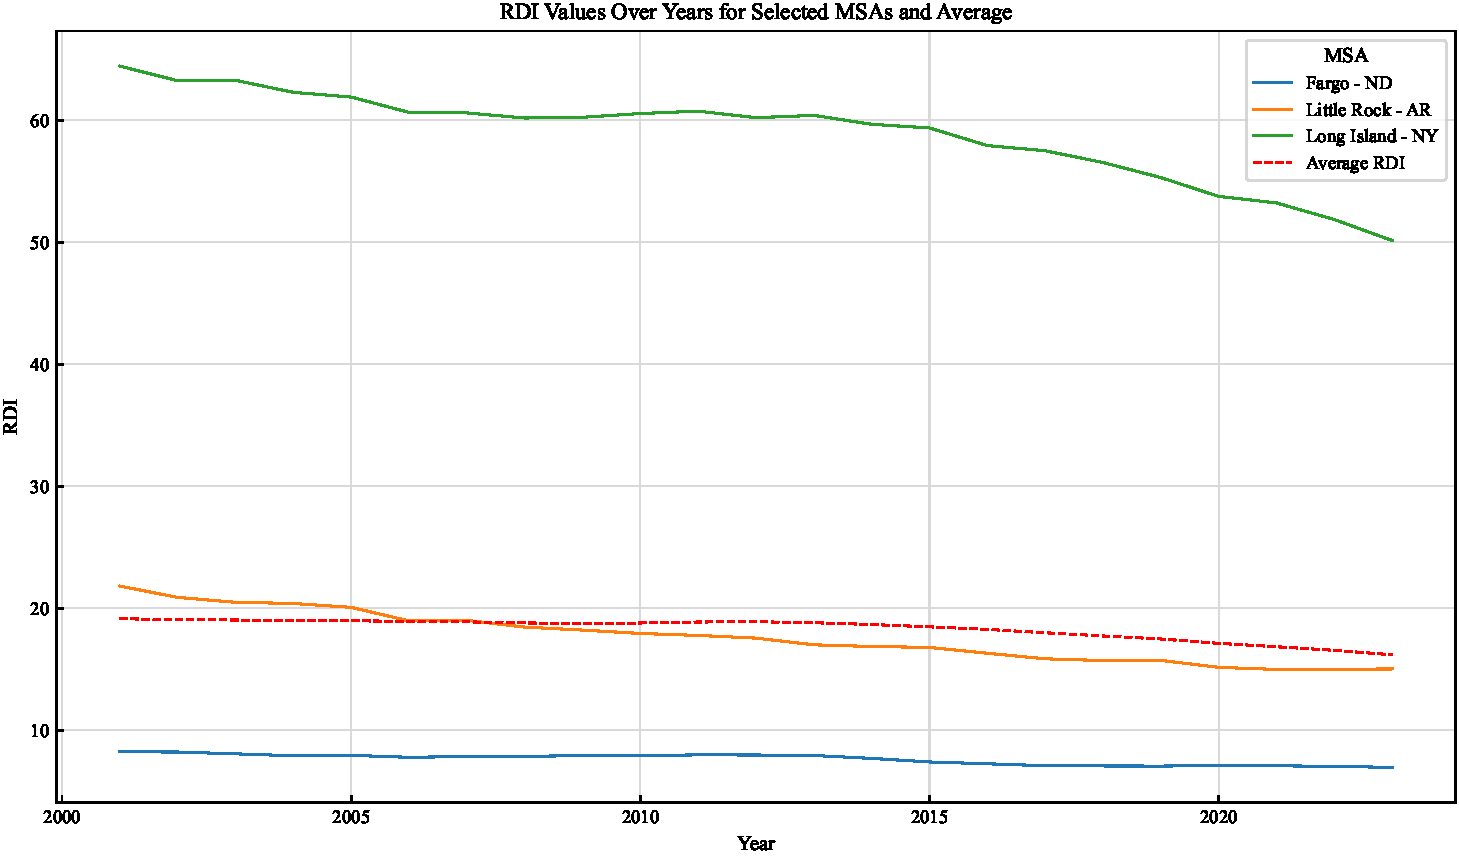
\includegraphics[width=\textwidth]{rdi_trends_selected_msas.pdf}
		\caption{A line graph showing the RDI values (population divided by apartment units) for the MSAs that were the min, max, and median in year 2001}
		\label{fig:rdi_lines}
	\end{subfigure}
	\caption{Histogram of Change in RDI, and Line Graph of RDI}
	\label{fig:sidebyside}
\end{figure}
This pattern poses a puzzle: if supply growth has outstripped population growth, why is everyone still worried about shortages? Occupancy simply tells you \textit{that} units are full--it cannot distinguish whether they are full by choice (everyone prefers roommates) or by necessity (everyone must share).

By contrast, year-over-year changes in RDI isolate the relative pace of new households versus new units. When rents rise faster than new construction can absorb, ΔRDI spikes, revealing latent demand pressure. When deliveries overwhelm demand, ΔRDI falls, signaling surplus. In the next section we exploit that property, regressing ΔRDI on rent and supply growth to recover the underlying demand curve.

\section{Empirical Framework}
Our objective is to evaluate \( \Delta \text{RDI} \) as a robust measure of housing demand by deriving supply and demand curves for each metropolitan area and year. For each of the 100 largest MSAs, and for each year from 2010 through 2022, we construct demand and supply curves using observed data on real rent per square foot and changes in RDI and supply.

\subsection{Constructing the Demand and Supply Curves}

We estimate reduced-form linear models to approximate demand and supply responses to price, using ten years of historical data for each MSA:
\begin{align*}
	\Delta \text{RDI}_{it} &= \alpha_i + \beta_i p_{it} + \epsilon_{it} && \text{(Demand)} \\
	\text{SupplyGrowth}_{it} &= \gamma_i + \delta_i p_{it} + \nu_{it} && \text{(Supply)}
\end{align*}

The coefficient \( \beta_i \) reflects how changes in rent induce renters to economize on space by cohabitating, while \( \delta_i \) captures developers' responsiveness to rent signals via new supply. We estimate these relationships using ordinary least squares (OLS) for each market-year observation, pooling data from the prior ten years. The intersection of these two curves yields the market's implied equilibrium rent \( p^* \) and equilibrium inventory growth \( q^* \). We compare these values to observed market outcomes \( (p, q) \) in that year. If \( p^* > p \), we infer that the market is underpriced; if \( p^* < p \), it is overpriced. Likewise, if \( q^* > q \), the market is deemed undersupplied; otherwise, oversupplied.The following pseudocode outlines the segmentation logic.
\FloatBarrier
\begin{algorithm}
	\caption{\enskip Segment markets into price–supply regimes (10‑year rolling window)}%
	\label{alg:market_segmentation}
	\begin{algorithmic}[1]
		\For{$y \gets 2010$ \textbf{to} 2022}
		\State $t_{\min}\gets \max(2010,\,y-10)$
		\For{each market $m$ in the top 100 MSAs}
		\State select data for $(m,t)$ with $t_{\min}\le t < y$
		\State fit demand: $\Delta\mathrm{RDI} = f(\mathrm{rent}_{psf})$ on years $t_{\min}\ldots y-1$
		\State fit supply: $\mathrm{inventory\ growth} = g(\mathrm{rent}_{psf})$ on the same years
		\State \textbf{solve for equilibrium} $(q^*,p^*)$ \textbf{by finding the price and quantity where}
		$f(p^*) = q^*$ \textbf{and} $g(p^*) = q^*$
		\State obtain actual values $(q,p)$ at year $y$
		\If{$q^* > q$}
		\If{$p^* > p$}
		\State assign $(m,y)\to\texttt{UndersuppliedUnderpriced}$
		\Else
		\State assign $(m,y)\to\texttt{UndersuppliedOverpriced}$
		\EndIf
		\Else
		\If{$p^* > p$}
		\State assign $(m,y)\to\texttt{OversuppliedUnderpriced}$
		\Else
		\State assign $(m,y)\to\texttt{OversuppliedOverpriced}$
		\EndIf
		\EndIf
		\EndFor
		\EndFor
	\end{algorithmic}
\end{algorithm}
\FloatBarrier
These states correspond to economic intuition. Overpriced and undersupplied markets---what we refer to as \textit{landlord-favorable} markets---are expected to exhibit stronger rent growth in the following year as prices can adjust faster than supply can be added. Conversely, oversupplied and underpriced markets---\textit{renter-favorable} markets---should experience weaker or negative rent growth for the same reason: prices can adjust faster than more people can arrive. The final two situations are partial disequilibria and their next year depends on which factor is more out of line with observed values. Overpriced and oversupplied markets are similar to late-cycle bubbles, while underpriced undersupplied markets are are similar to early-cycle growth. 

\begin{table}[h!]
	\centering
	\caption{Market Classification based on Observed versus Derived Prices and Quantities}
	\begin{tabular}{cc|c|c|}
		\multicolumn{2}{c}{} & \multicolumn{2}{c}{\textbf{Pricing}} \\
		\multicolumn{2}{c}{} & \textbf{Overpriced} & \textbf{Underpriced} \\
		\cmidrule{3-4}
		\multirow{2}{*}{\textbf{Supply}} & \textbf{Oversupplied} & Neutral-Late  & Renter-Favorable \\
		\cmidrule{2-4}
		& \textbf{Undersupplied} & Landlord-Favorable & Neutral-Early \\
		\bottomrule
	\end{tabular}
\end{table}


\subsection{Response to Shocks}
By way of example, we can look at a supply shock as experienced by Phoenix in 2022 (figure \ref{fig:phoenix_mechanism}). The supply line is constructed by regressing the change in supply and the real rent per-square-foot. The demand line is constructed by regressing the change in RDI and the real rent per-square-foot. Both use the data from 2012-2021. Their intersection (red circle) gives the implied 2021 market‑clearing rent (\$0.76 / sf) and inventory growth (0.74 \%). But the observed values are in 2022 (blue circle) were both greater greater than derived, so this market would be classified as overpriced and oversupplied, characteristics of a bubble. It is more overpriced than it is oversupplied, and so it returns to equilibrium through a price decline in the years that follow. 

\begin{figure}[htb!]
	\centering
	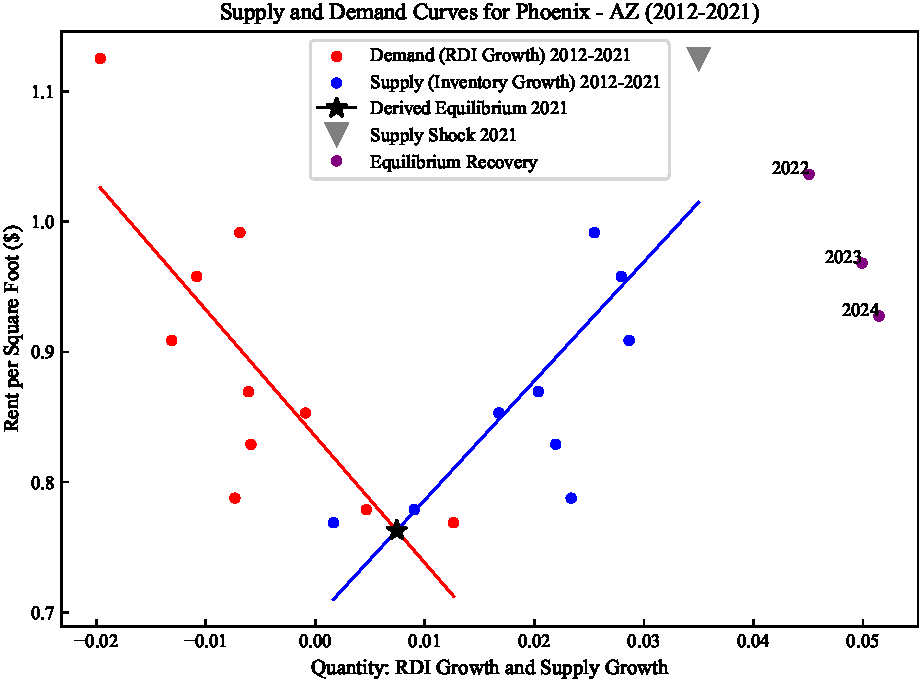
\includegraphics[width=0.95\linewidth]{phoenix_example.pdf}
	\caption{Recovering equilibrium for a high growth market.  
		Black circles: supply growth vs real rent 2012‑2022, Phoenix MSA.  
		Green circles: Rental‑Density‑Index growth (ΔRDI) vs real rent, same years.  
}
	\label{fig:phoenix_mechanism}
\end{figure}



We frame this as a partial equilibrium exercise, in which observed price and quantity may deviate from the implied market-clearing levels due to frictions such as construction lags, policy constraints, or imperfect price discovery \cite{wheaton1991realestate, glaeser2019rethinking}. This segmentation yields market classifications that form the basis for our predictive rent growth analysis in the following section.

\section{Results}

This section presents empirical findings from our market classification framework. Using the derived supply and demand curves, we compute equilibrium prices (\( p^* \)) and quantities (\( q^* \)) for each of the 100 largest MSAs from 2010 to 2022. By comparing \( (p^*, q^*) \) to the observed market outcomes \( (p, q) \), we segment markets into four states based on whether they are overpriced and/or oversupplied.

%PLACEHOLDER
%Fig 4 – 4‑quadrant heat‑map of all 100 MSAs (color = rent growth, size = inventory) for the latest year



\subsection{Statistical Tests of Group Differences}
We assess whether these classifications are associated with meaningful differences in future rent performance. Table \ref{tab:simplifiedmeans} reports average next-year relative real rent growth (defined as deviation from the within-year median) across the four groups formed by the boolean indicators `overpriced` and `oversupplied`.


	
%----------------------%
% Table of Group Means %
%----------------------%
\begin{table}[ht]
	\centering
	\caption{Group means, 95\% CIs, and one‐sided \(p\)–values}
	\label{tab:group_stats}
	\begin{tabular}{lrrrrr}
		\toprule
		Group & Mean Rent Growth (bps) & 95\% CI Lower & 95\% CI Upper & \(p\)–value & \(n\) \\
		\midrule
		Landlord-Favorable  &  94\(\,^{***}\) &   46 & 142 & 0.000276 &  63 \\
		Neutral-Early             &  25\(\,^{*}\)   &    6 &  45 & 0.010219 & 173 \\
		Neutral-Late         &  14             &   -5 &  33 & 0.150306 & 684 \\
		Renter‐Favorable    & -23\(\,^{***}\) &  -34 & -11 & 0.000110 & 380 \\
		\bottomrule
	\end{tabular}
	
	\vspace{0.5ex}
	\footnotesize{\(^{*}p<0.05\), \(^{**}p<0.01\), \(^{***}p<0.001\) (one‐sided test vs.\ 0).}
\end{table}

Examining the average relative real rent growth of the different groups shows the significance of the demand variable and its classification system. When markets are out of equilibrium (Landlord-Favorable or Renter-Favorable) we see significant and opposite responses in the following year real relative rent growth. The year after a market is classified as Landlord-Favorable it has real relative rent growth of between 42 and 142 basis points. This is in addition to the nominal rent growth and to the median rent growth of the top markets. Thus if median rent growth were 3\% in that year, Landlord-Favorable markets saw rent growth of 3.94\%. Conversely, the year after a market is classified as Renter-Favorable, it has negative relative real rent growth. 
It is worth noting that the two Neutral groups have confidence intervals that include zero --hence the low significance. But this is precisely what one expects to see from markets in partial equilibrium: their relative real rent growth is not significantly different from zero (or the median in our case, as we standardized th values to the median annual rent growth).

%----------------------%
% Two-Way ANOVA Table  %
%----------------------%
\begin{table*}[t]
	\centering
	\begin{threeparttable}
		\caption{Two-Way ANOVA\label{tab:anova}}
		\begin{tabular}{lcccc}
			\toprule
			Source              & Sum Sq   & df    & $F$      & PR($>F$) \\
			\midrule
			C(overpriced)       & 0.005178 & 1.0   & 12.311490$^{***}$  & 0.000466 \\
			C(oversupplied)     & 0.006205 & 1.0   & 14.751522$^{***}$  & 0.000129 \\
			Residual            & 0.545538 & 1297.0& ---      & --- \\
			\bottomrule
		\end{tabular}
		\begin{tablenotes}
			\footnotesize
			\item Note: *** $p<0.01$, ** $p<0.05$, * $p<0.10$. Robust standard errors are used.
		\end{tablenotes}
	\end{threeparttable}
\end{table*}

The two-way ANOVA reports that there are significant differences between the overpriced and underpriced groups; and so too with the oversupplied and undersupplied groups.

%-----------------------------%
% Tukey HSD Post-Hoc Test     %
%-----------------------------%
\begin{table*}[t]
	\centering
	\begin{threeparttable}
		\caption{Tukey HSD Post-Hoc Test\label{tab:tukey}}
		\begin{tabular}{lcccccc}
			\toprule
			\multicolumn{1}{c}{Group1} & Group2             & Mean Diff & p-adj  & Lower  & Upper & Reject Null\\
			\midrule
			Neutral-Early               & Landlord-Favorable  & 0.0069   & 0.1012 & -0.0009 & 0.0147  & False \\
			Neutral-Early               & Neutral-Late         & -0.0012  & 0.9082 & -0.0057 & 0.0033  & False \\
			Neutral-Early              & Renter-Favorable    & -0.0049  & 0.0468 & -0.0097 & -0.0000 & True  \\
			Landlord-Favorable    & Neutral-Late         & -0.0081  & 0.0150 & -0.0150 & -0.0011 & True  \\
			Landlord-Favorable    & Renter-Favorable    & -0.0118  & 0.0001 & -0.0190 & -0.0046 & True  \\
			Neutral-Late           & Renter-Favorable    & -0.0037  & 0.0243 & -0.0071 & -0.0003 & True  \\
			\bottomrule
		\end{tabular}
		\begin{tablenotes}
			\footnotesize
			\item Note: The Tukey HSD Post-Hoc Test compares mean differences between groups at a family-wise error rate (FWER) of 0.05. 
		\end{tablenotes}
	\end{threeparttable}
\end{table*}

Examining the differences between the means of the classifications shows that Neutral-Early markets are not significantly different from others-- the upper bound of the CI of the comparison to Renter-Favorable barely excludes zero. But all other comparisons were significantly different, with the Lanlord-Favorable markets 118 basis points higher in mean relative real rent than the Renter-Favorable markets. 

To aid interpretation, Table~\ref{tab:matrixlabels} maps the binary groups to intuitive market types.

\begin{table}[h!]
	\centering
	\caption*{Market Classification by Pricing and Supply}
	\label{tab:matrixlabels}
	\begin{tabular}{cc|c}
		\toprule
		\textbf{Overpriced} & \textbf{Oversupplied} & \textbf{Label} \\
		\midrule
		False & False & Balanced Market \\
		False & True & Renter-Favorable \\
		True  & False & Landlord-Favorable \\
		True  & True  & Price Bubble \\
		\bottomrule
	\end{tabular}
\end{table}

These results support our core hypothesis: landlord-favorable markets exhibit the strongest subsequent rent growth, while renter-favorable markets experience the weakest. Balanced and bubble-like markets show intermediate outcomes.





These patterns do not appear in the raw rent growth values, reinforcing that our framework is best applied in relative terms—benchmarking each MSA against its peers in a given year.
\subsection{Event Study: Rent Growth Before and After Regime Entry}

To complement our classification-based forecasting approach, we implement an event study that traces rent dynamics around the time a market enters the \emph{Overpriced \& Oversupplied} regime. This regime—characterized by both above-equilibrium rents and excessive new supply—is hypothesized to precede periods of slower rent growth or correction. 

We define the event year $t=0$ as the first year an MSA is classified as Overpriced \& Oversupplied. We construct an event time index ranging from $t = -2$ (two years before the regime entry) to $t = +2$ (two years after entry). For each event-time year, we compute the average real rent growth across all MSAs that experienced the regime switch.

This structure ensures that the rent growth observed at $t+1$ and $t+2$ is entirely out-of-sample with respect to the classification year $t=0$. To contextualize the results, we compare these patterns to MSAs that never entered the Overpriced \& Oversupplied regime during the study period, as well as to those that experienced alternative classification transitions.

%PLACEHOLDER
%INCLUDE THE RESULTS VS ARIMA AND NAIVE MODELING
Figure~\ref{fig:event_study} displays average real rent growth by event year for each group.

\begin{figure}[h]
	\centering
	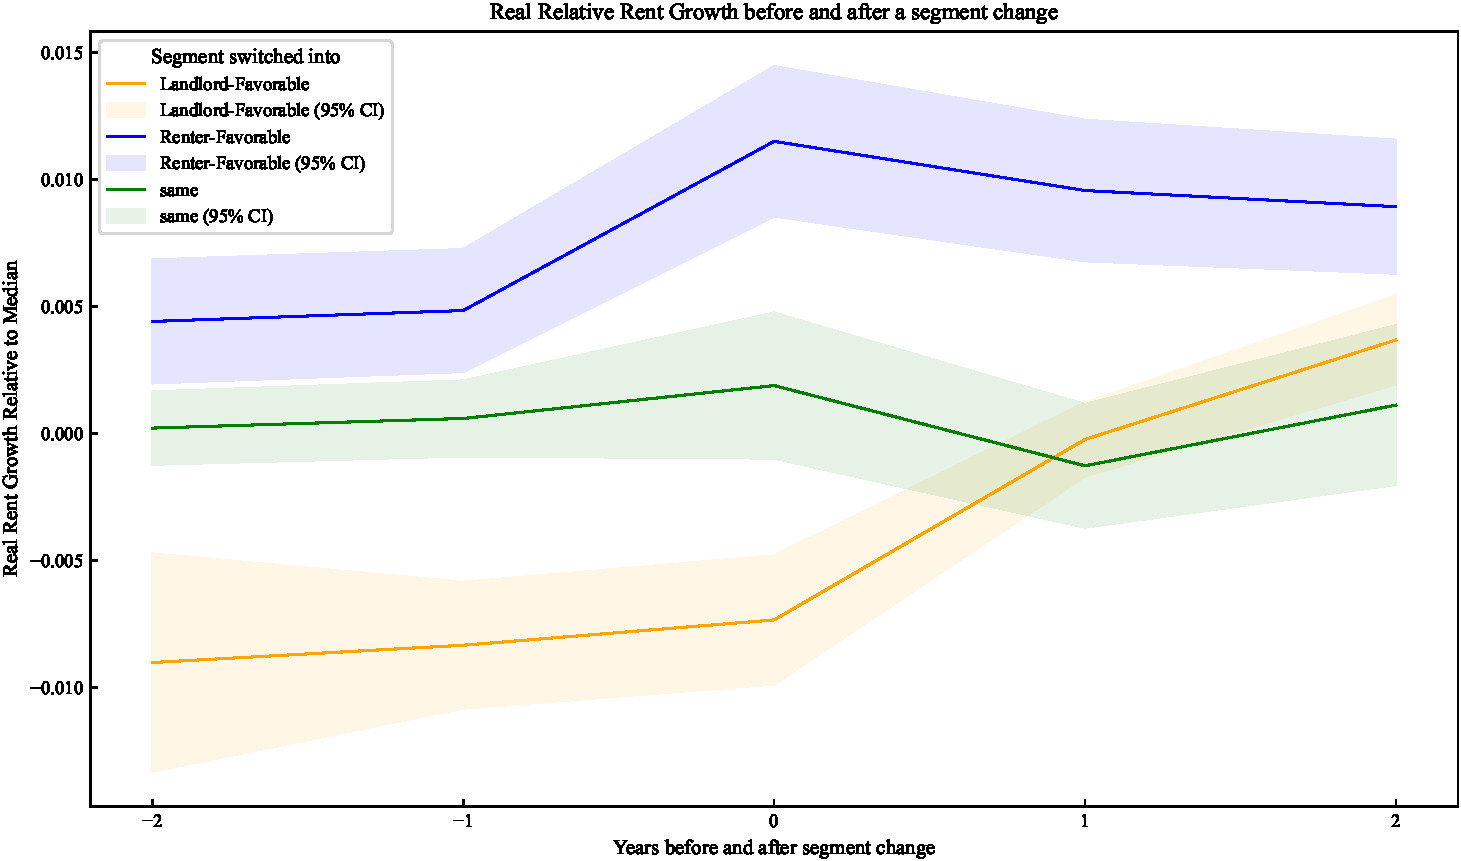
\includegraphics[width=0.8\textwidth]{event_study.pdf}
	\caption*{Event study of average real rent growth before and after entry into the Overpriced \& Oversupplied regime ($t=0$).}
	\label{fig:event_study}
\end{figure}

The results show that real rent growth slows meaningfully following entry into the Overpriced \& Oversupplied regime. While pre-entry years may exhibit moderate rent growth, the post-entry period is characterized by significantly lower average rent changes. This pattern supports the hypothesis that this classification regime is forward-looking and useful in anticipating market cooling or correction.

\subsection{Visual and Quantitative Robustness}



Figure~\ref{fig:group_averages_over_time} shows the average real rent in the landlord and renter-favorable markets, as classified the prior year, highlighting the predictive spread between groups.

\begin{figure}[h]
	\centering
	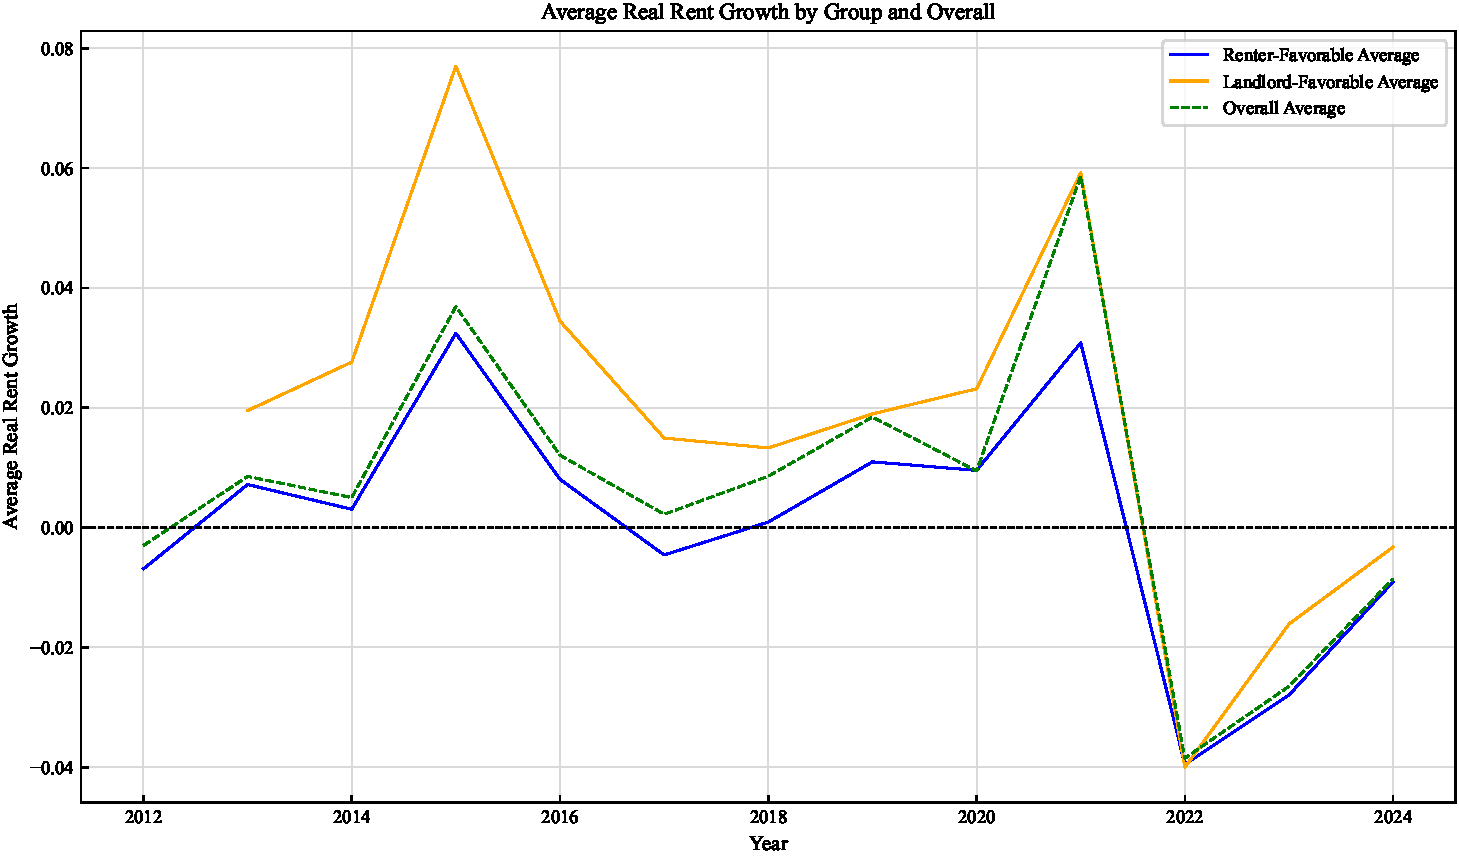
\includegraphics[width=0.8\textwidth]{group_averages_over_time.pdf}
	\caption*{Each market was classified in the prior year ($t-1$); the real rent growth shown is for the following year ($t$)}
	\label{fig:group_averages_over_time}
\end{figure}


The landlord-favorable group exceeds the renter-favorable group by, on average, 163 basis points, which is just over one standard deviation, reinforcing the economic magnitude of these classification effects.

\subsection{Distributional Evolution and Market Cycles}

Here we take a meta-examination of the classification system. The groupings are not evenly distributed across years, as we did not enforce a normalization. Instead, this reflects underlying market behavior rather than methodological bias. 

\begin{table}[ht]
	\centering
	\caption{Market Classification and Average Real Rent Growth (2011--2024)}
	\label{tab:market_rent_growth}
	\begin{tabular}{lccccc}
		\toprule
		Year & Neutral-Early & Renter-Friendly & Landlord-Friendly & Neutral-Late & Avg. Real Rent Growth \\
		\midrule
		2011 & 61\% & 0\%  & 36\% & 3\%  & -2\% \\
		2012 & 36\% & 2\%  & 60\% & 2\%  & 0\%  \\
		2013 & 26\% & 2\%  & 67\% & 5\%  & 1\%  \\
		2014 & 22\% & 1\%  & 64\% & 13\% & 1\%  \\
		2015 & 9\%  & 7\%  & 38\% & 46\% & 4\%  \\
		2016 & 4\%  & 8\%  & 26\% & 62\% & 1\%  \\
		2017 & 3\%  & 7\%  & 22\% & 68\% & 0\%  \\
		2018 & 2\%  & 6\%  & 17\% & 75\% & 1\%  \\
		2019 & 2\%  & 6\%  & 7\%  & 85\% & 2\%  \\
		2020 & 1\%  & 5\%  & 6\%  & 88\% & 1\%  \\
		2021 & 0\%  & 8\%  & 3\%  & 89\% & 6\%  \\
		2022 & 2\%  & 8\%  & 13\% & 77\% & -4\% \\
		2023 & 5\%  & 3\%  & 21\% & 71\% & -3\% \\
		2024 & 2\%  & 8\%  & 30\% & 60\% & -1\% \\
		\bottomrule
	\end{tabular}
\end{table}


In early years such as 2011, few MSAs exhibit characteristics of overpriced and oversupplied markets, consistent with post-crisis housing conservatism. By contrast, between 2020 and 2022, the vast majority of MSAs fall into the “Price Bubble” category, despite negative or flat rent growth. This asymmetry suggests the framework captures real cyclical shifts, where high observed rents and heavy supply growth outpace renter willingness or ability to absorb space. The sharp contrast between high pricing and poor performance in these years further reinforces the framework’s value in signaling impending cooling phases or market corrections.

\subsection{Predictive Power and Caveats}

To gauge if the predictive power offered by the model is significant, we compare it to the forecasts of an ARIMA model and a naive model. The ARIMA model looks at trailing-10 year periods and forecasts the next year. The naive model assumes that the markets that were the top performers in the prior year will continue to be top performers in the following year. We then take the average rent growth of the forecasted top third and subtract it from the average rent growth of the forecasted bottom third.

\begin{figure}[h]
	\centering
	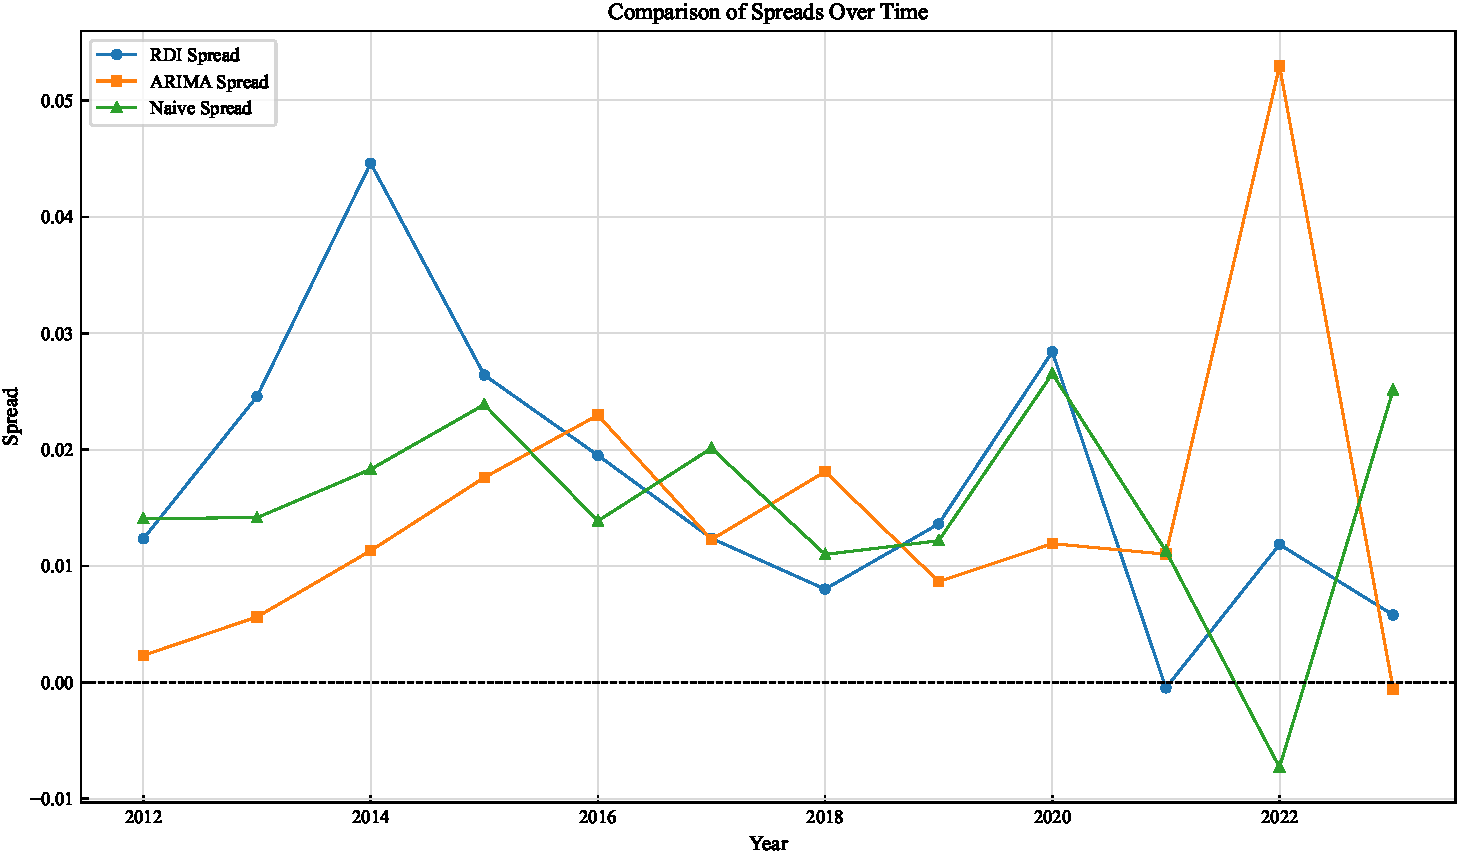
\includegraphics[width=0.8\textwidth]{spread_comparison_over_time.pdf}
	\caption*{Event study of average real rent growth before and after entry into the Overpriced \& Oversupplied regime ($t=0$).}
	\label{fig:event_study}
\end{figure}


The relative-density system had a spread of 172 basis points between its Landlord-Favorable and Renter-Favorable markets. The ARIMA model had a spread of 145 basis points, while the naive model had a spread of 153 basis points. This suggests the implied demand signal can be used to rank markets by expected future performance, offering both interpretability and predictive power.

While this forecasting result is encouraging, we acknowledge a potential limitation: market pricing and supply choices may themselves reflect expectations about future rent growth. This opens the door to endogeneity. Although our model uses trailing 10-year trends to construct classifications, future work should explore this causal directionality more rigorously.

Together, these findings validate the informational value of market misalignment relative to derived equilibrium, offering a parsimonious and predictive classification of multifamily rent dynamics.

\begin{table}[ht]
	\centering
	\caption{Yearly Spread Comparison}
	\label{tab:yearly_spread}
	\begin{tabular}{lccc}
		\toprule
		Year & RDI Spread & ARIMA Spread & Naive Spread \\
		\midrule
		
		2012 & 0.0123     & 0.0023      & 0.0141     \\
		2013 & 0.0246     & 0.0056      & 0.0141     \\
		2014 & 0.0446     & 0.0113      & 0.0183     \\
		2015 & 0.0264     & 0.0176      & 0.0239     \\
		2016 & 0.0195     & 0.0230      & 0.0139     \\
		2017 & 0.0124     & 0.0123      & 0.0201     \\
		2018 & 0.0080     & 0.0181      & 0.0110     \\
		2019 & 0.0136     & 0.0087      & 0.0122     \\
		2020 & 0.0284     & 0.0119      & 0.0265     \\
		2021 & -0.0005    & 0.0110      & 0.0113     \\
		2022 & 0.0118     & 0.0530      & -0.0073    \\
		2023 & 0.0058     & -0.0006     & 0.0251     \\
		
		\bottomrule
	\end{tabular}
\end{table}

\begin{table}[ht]
	\centering
	\caption{Average Spread Comparison}
	\label{tab:average_spread}
	\begin{tabular}{lc}
		\toprule
		Variable & Average Value \\
		\midrule
		
		RDI Spread & 0.0172 \\
		ARIMA Spread & 0.0145 \\
		Naive Spread & 0.0153 \\
		\bottomrule
	\end{tabular}
\end{table}



\section{Discussion}

Our findings reinforce the utility of rental density---measured as population per occupied rental unit---as a robust proxy for demand in multifamily housing markets. Traditional demand-side variables such as occupancy and absorption are bounded above by 100\%, rendering them structurally incapable of expressing excess demand. By contrast, our proposed measure, the change in Rental Density Index (\(\Delta\text{RDI}\)), accommodates marginal and nonlinear shifts in tenant behavior, particularly around unit sharing or household formation.

The empirical evidence supports this theoretical proposition. When supply and demand curves were derived from historical \(\Delta\text{RDI}\) and supply growth data, we observed that the relative position of actual market conditions to the implied equilibrium---quantified as overpriced/underpriced and oversupplied/undersupplied---was significantly associated with next-year rent growth. Specifically, markets that were both overpriced and undersupplied experienced statistically higher rent growth than other combinations. Conversely, renter-favorable markets (underpriced and oversupplied) exhibited lower growth or even declines. 

This segmentation has both explanatory and predictive power. Our simplified ANOVA model revealed statistically significant differences in next-year rent growth across these market states. We presented an event-study model showing the impact of being classified as 'Renter-Friendly' and 'Landlord-Friendly' in the years following the classification. Finally we compared the predictive power of our classification system to that of ARIMA models and naive models used to forecast market rent-growth. In this comparison as well, our model outperformed. 

While the number of MSAs in each state was not evenly distributed across years, this asymmetry reflects genuine market dynamics rather than bias or misclassification. For example, in periods of expansion, we naturally observe more overpriced or undersupplied markets, consistent with cyclical pressures on housing. Nonetheless, even in years with few markets in a given segment, those groupings consistently displayed expected behavior in rent trajectories.

These findings reinforce the value of \(\Delta\text{RDI}\) as a continuous, forward-looking measure of housing demand, especially when contrasted with backward-looking or constrained alternatives. They also suggest that equilibrium misalignment---in both price and quantity---can be quantified in a way that is both actionable for investors and meaningful for policymakers.

\section{Conclusion}

This paper contributes to the literature on housing market dynamics by introducing the change in Rental Density Index (\(\Delta\text{RDI}\)) as a scalable, interpretable measure of demand. Unlike occupancy or absorption, \(\Delta\text{RDI}\) captures variation in consumer preference through household formation behavior---a critical but often overlooked channel of adjustment in rental markets.

By modeling supply and demand curves separately and estimating their intersection, we were able to derive implied market-clearing quantities and prices for each metropolitan area in our dataset. These derived values allowed for the segmentation of MSAs into four quadrants based on price and supply misalignment. Across the 100 largest U.S. markets from 2010 to 2023, these quadrants were statistically associated with next-year rent growth in ways consistent with theory: undersupplied and overpriced markets performed best; oversupplied and underpriced markets performed worst.

This demand proxy also showed moderate predictive power when used in a linear forecasting framework, suggesting that it may serve as a leading indicator of rent pressure---particularly when combined with supply metrics. The ability to anticipate future rent dynamics is valuable to developers, institutional landlords, and policymakers seeking to manage affordability and stability in rental housing.

Future work should explore refinement of \(\Delta\text{RDI}\) to account for compositional changes in renter populations and household structures. Additional improvements might include the integration of MSA-specific CPI indices or disaggregated demand inputs, such as migration, income distributions, or age cohorts. Nonetheless, the present analysis establishes \(\Delta\text{RDI}\) as a conceptually valid and empirically useful measure of multifamily housing demand, with applications in forecasting, pricing, and supply planning.


%\backmatter
\bmsection*{Author contributions}

This is an author contribution text. This is an author contribution text. This is an author contribution text. This is an author contribution text. This is an author contribution text.

\bmsection*{Acknowledgments}
 here. This is acknowledgment text. Provide text here. This is acknowledgment text. Provide text here. This is acknowledgment text. Provide text here. This is acknowledgment text. Provide text here.


\bmsection*{Financial disclosure}

None reported.

\bmsection*{Conflict of interest}

The authors declare no potential conflict of interests.
\bibliography{wileyNJD-APA}
\bmsection*{Supporting information}

Additional supporting information may be found in the
online version of the article at the publisher’s website.






\begin{lstlisting}[caption={Descriptive caption text},label=DescriptiveLabel, basicstyle=\fontsize{8}{10}\selectfont\ttfamily]
for i:=maxint to 0 do
begin
{ do nothing }
end;
Write('Case insensitive ');
WritE('Pascal keywords.');
\end{lstlisting}




\nocite{*}% Show all bib entries - both cited and uncited; comment this line to view only cited bib entries;


\bmsection*{Author Biography}

\begin{biography}{
\includegraphics[width=76pt,height=76pt,draft]{empty}}{
{\textbf{Author Name.} Please check with the journal's author guidelines whether
author biographies are required. They are usually only included for
review-type articles, and typically require photos and brief
biographies for each author.}}
\end{biography}


\end{document}
